\documentclass[11pt]{report}
\usepackage{titlesec}
\titleformat{\chapter}
{\filcenter\normalfont\Large\bfseries}
{\chaptertitlename~\thechapter} {0.5em} {}

\usepackage[english]{babel}
\usepackage{graphicx}
\usepackage{amsmath,amssymb}
\usepackage{bbm}
\usepackage{listings} %listing R code
\usepackage{siunitx} %voor 10^
\usepackage[usenames,dvipsnames]{color}
\usepackage{color}
\usepackage{enumitem}
\usepackage{pdfpages}
\usepackage{titling}
\usepackage{hyperref}

\usepackage{amssymb}

\usepackage[T1]{fontenc}
\usepackage[utf8]{inputenc}
\usepackage{charter}
\usepackage{environ}
\usepackage{tikz}
\usetikzlibrary{calc,matrix}

%%%%%%%%%%%%%%%%%%%%%%%%%%%%%%%%
% code by Andrew:
% http://tex.stackexchange.com/a/28452/13304
\makeatletter
\let\matamp=&
\catcode`\&=13
\makeatletter
\def&{\iftikz@is@matrix
  \pgfmatrixnextcell
  \else
  \matamp
  \fi}
\makeatother

\newcounter{lines}
\def\endlr{\stepcounter{lines}\\}

\newcounter{vtml}
\setcounter{vtml}{0}

\newif\ifvtimelinetitle
\newif\ifvtimebottomline
\tikzset{description/.style={
  column 2/.append style={#1}
 },
 timeline color/.store in=\vtmlcolor,
 timeline color=red!80!black,
 timeline color st/.style={fill=\vtmlcolor,draw=\vtmlcolor},
 use timeline header/.is if=vtimelinetitle,
 use timeline header=false,
 add bottom line/.is if=vtimebottomline,
 add bottom line=false,
 timeline title/.store in=\vtimelinetitle,
 timeline title={},
 line offset/.store in=\lineoffset,
 line offset=4pt,
}

\NewEnviron{vtimeline}[1][]{%
\setcounter{lines}{1}%
\stepcounter{vtml}%
\begin{tikzpicture}[column 1/.style={anchor=east},
 column 2/.style={anchor=west},
 text depth=0pt,text height=1ex,
 row sep=1ex,
 column sep=1em,
 #1
]
\matrix(vtimeline\thevtml)[matrix of nodes]{\BODY};
\pgfmathtruncatemacro\endmtx{\thelines-1}
\path[timeline color st] 
($(vtimeline\thevtml-1-1.north east)!0.5!(vtimeline\thevtml-1-2.north west)$)--
($(vtimeline\thevtml-\endmtx-1.south east)!0.5!(vtimeline\thevtml-\endmtx-2.south west)$);
\foreach \x in {1,...,\endmtx}{
 \node[circle,timeline color st, inner sep=0.15pt, draw=white, thick] 
 (vtimeline\thevtml-c-\x) at 
 ($(vtimeline\thevtml-\x-1.east)!0.5!(vtimeline\thevtml-\x-2.west)$){};
 \draw[timeline color st](vtimeline\thevtml-c-\x.west)--++(-3pt,0);
 }
 \ifvtimelinetitle%
  \draw[timeline color st]([yshift=\lineoffset]vtimeline\thevtml.north west)--
  ([yshift=\lineoffset]vtimeline\thevtml.north east);
  \node[anchor=west,yshift=16pt,font=\large]
   at (vtimeline\thevtml-1-1.north west) 
   {\textsc{Timeline \thevtml}: \textit{\vtimelinetitle}};
 \else%
  \relax%
 \fi%
 \ifvtimebottomline%
   \draw[timeline color st]([yshift=-\lineoffset]vtimeline\thevtml.south west)--
  ([yshift=-\lineoffset]vtimeline\thevtml.south east);
 \else%
   \relax%
 \fi%
\end{tikzpicture}
}
%%%%%%%%%%%%%%%%%%%%%%%%%%%%%%%%

\newcommand{\half}{\frac{1}{2}}
\newcommand{\pref}[1]{(\ref{#1})}
\newcommand{\itab}[1]{\hspace{0em}\rlap{#1}}
\newcommand{\tab}[1]{\hspace{.4525\textwidth}\rlap{#1}}

\pretitle{%
  \begin{center}
  \LARGE
  
\includegraphics[width=11.35cm]{./Attachments/logoAAPP16}\\[\bigskipamount]
}
\posttitle{\end{center}}

\title{AAPCie Guide}
\author{STORM}
\date{\today}

%%%%%%%%%%%%%%%%%%%%%%%%%%%%%%%%%%

\begin{document}
\selectlanguage{english}
\maketitle
\tableofcontents
\clearpage

\chapter{Definitions}
\begin{description}
\item[AAPP:]
De Amsterdam Algorithm Programming Preliminaries, wordt ook wel gerefereerd in het document als de contest. De contest wordt georganiseerd door Studievereniging STORM en is bedoeld voor alle VU studenten. Het vindt plaats midden/eind september. AAPP geldt als voorronde voor de BAPC.

\item[BAPC:]
De Benelux Algorithm Programming Contest, georganiseerd door een studievereniging in de Benelux. Het vindt meestal plaats eind oktober. BAPC geldt vanaf $2016$ als voorronde voor NWERC.

\item[NWERC:]
De Northwestern Europe Regional Contest. Het vindt plaats eind november. NWERC geldt als de voorronde voor de ICPC World Finales.

\item[ICPC World Finales]
De International Collegiate Programming Contest (ICPC) World Finales is de wereld finale, die rond maart wordt gehouden.

\item[Organisatie:]
De leden van de organiseerde commissie van STORM, ook wel de AAPPCie genoemd.

\item[Website:]
Wordt onderhouden door de organisatie en bevat onder andere informatie, problems van vorige jaren en de regels van de AAPP. De website is beschikbaar op \url{http://www.storm.vu/aapp}.

\item[Jury:]
Groep mensen die verantwoordlijk zijn voor het controleren van de antwoorden op de submission van deelnemers.

\item[Tech:]
Groep mensen die verantwoordlijk zijn voor het systeem.

\item[Balloon girls:]
Runners die verantwoordlijk zijn voor het uitdelen van printjes, het beantwoorden van vragen en het uitdelen van ballonen aan teams die een submission correct hebben ingeleverd.

\item[Crew:]
Organisatie, leden van de jury, tech en balloon girls. 

\item[Deelnemers:]
Leden van een deelnemende team die meedoen aan de contest.

\item[Submission:]
De submission van een oplossing door een team, welke ingeleverd kan worden via DomJudge  en die gecontroleerd zal worden door onze nakijkservers.
\end{description}

\chapter{How does a programming contest works?}
\section{Preliminaries}
For students of the VU Amsterdam, the International Collegiate Programming Contest (ICPC) knows four rounds:
\begin{enumerate}
\item Amsterdam Algorithm Programming Preliminaries (AAPP): Open for all VU Amsterdam teams which satifsy the conditions, see also the Appendix \ref{EligibilityDecisionTree}. The top three teams are allowed to BAPC.
\item Benelux Algorithm Programming Contest (BAPC): The top three teams of each educational institution can accompete to BAPC. The top two teams of  each educational institution are allowed to NWERC, provided that the team consists three team members (see also Appendix \ref{EligibilityDecisionTree}).
\item Northwestern Europe Regional Contest (NWERC): The top two teams of each educational institution can accompete to NWERC. The top three teams of  each educational institution are allowed to the ICPC World Finales.
\item International Collegiate Programming Contest (ICPC) World Finales: The top three teams of the region Northwestern Europe are allowed to the ICPC World Finals.
\end{enumerate}
Teams that do not satisfy the Eligibility Decision Tree (see appendix \ref{EligibilityDecisionTree}), are usually allowed as spectator if there is room for them.

\section{General Concept of the Contest}
Each team (with a maximum of three students) is trying to solve as many problems (most of the time between the $10$ and the $13$) as possible in five hours, by programming a program on the computer. The program reads the input from the input file, search or computes the right answer and gives back the results as output.

Most of the time, the problems are based on known classic algorithms, like the shortest path algorithm of Dijkstra or backtracking. Often there are a number of mathematical problems.

Logically, may only discuss with their teammates. Furthermore, it is allowed to use a cheat sheet (Team Reference Document) and to bring their own keyboard. Teams that have a problem correctly within four hours, gets a balloon of a balloon babe in the color of the problem.

\section{Sending in a Submissions}
Via the jury interface DomJudge (a website), teams can hand in the submissions. Further access to the internet has been blocked during the contest. The jury interface also tells the teams, if the submissins was correct or not. The program will be rated on the following two criteria: accuracy and efficiency.

That means: the program has solve a set of test cases (not only the one given as input in the problem) in previously set time limit (most of the time a few secondes).

The following reactions of the jury are possible:
\begin{itemize}
\item Accepted;
\item Wrong Answer;
\item Timelimit Exceeded;
\item Runtime Error.
\end{itemize}
For each correct solution (Accepted), you will get a balloon from a balloon babe (if the correct solution was hand in within the first four hours).

\section{Program languages}
The following program languages are accepted at the contest:
\begin{itemize}
\item[AAPP] Java, C, C++, Python
\item[BAPC] Java, C, C++
\item[NWERC] Java, C,  C++
\item[ICPC World Finales] Java, C, C++
\end{itemize}

\section{Score}
The team score depends on two parts:
\begin{itemize}
\item The number of correct solved problems within the five hours
\item The total time (including the penalty time).
\end{itemize}
%
There are two parts per solved problem:
\begin{itemize}
\item The numbers of minutes since the start of the contest and the moment till solving the problem %Het aantal minuten tussen het begin van de wedstrijd en het oplossen van de opgave
\item $20$ minutes penalty time for each wrong solution %strafminuten voor elke foute inzending
\end{itemize}
A wrong solution only gives penalty time if the problem is solved later the contest.

On the scoreboard, teams will be sorted by the numbers of solved problems. Teams who has same amount of solved problems, will be sorted on total time. In the last hour of the contest, the scoreboard will be freezed. You will see from your own team if a problem is correct or not, but it is not possible to see on the scoreboard if others teams have hand in a (correct) solution.

See for more information the rulebook, Appendix \ref{Rulebook} (Judgement).

\section{Time Schedule}
Each program contest has the same set up when its come to time. Some organisations decided to spread this event over a weekend, to create some room for excursions and sponsoring activities. This is the case at NWERC, since teams are coming from foreign countries. However, teams likely do not like it that it takes that long before they can really start with the contest.

The time schedule for the contest is as follow:
\subsection{Registration (total time: $30$ - $40$ minutes)}
Registration of the incoming teams. Showing up as a full team is very practical instead of showing up as an indiviual team member. The organisation handout the following things to the teams (and there coach):
\begin{itemize}
\item Finale remark sheet (advice, hints and general information from the jury);
\item Goodiebags (most of the time including pens, promotion flyers, a contest book and a mug/cup with the organisation logo on it);
\item Sponsored T-shirt, which we are mandatory to wear during the day(s) or contest;
\item Name badges (including teamname).
\end{itemize}
\textbf{Tip: Most of the organisations provide some coffee and tea since the registrations are always early in the morning.}

The teams need to hand in the following things to the organisation:
\begin{itemize}
\item Keyboard (one per team, wireless is not accepted)
\item Cheatsheets (maximum of $3$ per team)
\end{itemize}

Furthermore, the organisation can:
\begin{itemize}
\item Check if there are any teammembers who are allergic for some kind of food and forgot to mention this to the organisation;
\item Control if there is any missing information in ICPC;
\item Take a beautiful team picture (which can be show at the Award Ceremony).
\end{itemize}

\subsection{Opening Ceremony (total time: $30$ minutes)}\label{openingCeremony}
Teams are being welcomed by the chairman or the contest director, and sometimes the main sponsor.

The following things can be mention at the introduction presentation:
\begin{itemize}
\item Statistics about numbers of
	\begin{itemize}
	\item Student;
	\item Teams;
	\item Universities;
	\item Countries
	\end{itemize}
compared to last year;
\item Time schedule of the day/weekend, and if there are any questions about that;
\item That it's mandatory to wear the T-shirt during the contest;
\item The rules of the contest;
\item Introducing the:
	\begin{itemize}
	\item Organisation;
	\item Jury;
	\item Balloon Babes;
	\item Main sponsor
	\end{itemize}
to the teams with names, pictures and there T-shirt color;
\item Welcome speech by the main sponsor.
\end{itemize}

\subsection{System Introduction (total time: $30$ minutes)}
Short presentation about the system, it is more convenient for a Tech member to give this presenation. The following things can be mention at the introduction presentation:
\begin{itemize}
\item What teams can bring on the contest floor;
\item Overview of what teams can use for there submissions, such as
	\begin{itemize}
	\item Accepted language;
	\item Compiler;
	\item Version;
	\item Flags;
	\end{itemize}
\item How the test session will work (and that there in an envelope);
\item Short questions about the system.
\end{itemize}

\subsection{Test session (total time: $60$ minutes)}
Before the contest starts, there is a test session to get used to the system. The problems are in an envelope which can be opened when the organisation said so. This test session is used to see if the contest environment fulfills all the expectations of the organisation and the participants.

\subsection{Coach meeting (total time: $60$ minutes)}
Meeting for the coaches, which can be held during the test session or the contest. See also section \ref{CoachMeeting} for more inside information.

\subsection{Lunch (total time: $60$ minutes)}
Lunch, most of the time catered by the main sponsor.

\subsection{Last remarks (total time: $30$ minutes)}\label{lastRemarks}
The latest issues will be discussed and the last questions of teams will be answered. Takes maximum a quarter of an hour, but we take $30$ minutes into account so that everybody has the time to take there seat at the contest floor before the contest starts.

\subsection{Contest (total time: $300$ minutes)}
Contest starts ($5$ hours), only the participants and the organisation are allowd on the contest floor. Coaches need to wait in the coach room.

\subsection{Freeze scoreboard (total time: $60$ minutes)}
Scoreboard is freezed. Teams can only see there own submission and if they are correct on the scoreboard. The judges can see the realtime scoreboard, while the coaches see the freezed version.

\subsection{Drinks (total time: $60$ minutes)}
Drinks after the contest, to pass time untill the award ceremony starts.

\subsection{Award ceremony (total time: $10$ minutes)}\label{awardCeremony}
Final score board will be present and the prizes will be handed out at the award ceremony.

\subsection{Presentation problems (total time: $15$ minutes)}
Presentation with solutions, which will be presented by the judges.

\subsection{Optional: Dinner}
Depends if the organisation has the money to compensate the cost for the participants.

\chapter{Committee Tasks}
\label{Functieverdeling}
\section{Chairman}
	Leads the commission and ensures that everything runs smoothly. He delegates and motivates the members of the commission to do there tasks (see also section \ref{motivated}). He also leads the meetings (see also section \ref{leadingMeetings}). Carries responsibility for the committee. \label{responsibilityChairman} Read also the responsibility of a contest director: \ref{responsibilityChairman}.
	
	\subsection{Leading the Meetings}\label{leadingMeetings}
	Plan regular meetings, but only do so when its \underline{necessary} because nobody likes pointless meetings. Make sure everyone gets the chance to bring something up during the meeting.
	
	Design for the agenda is as follow (Dutch/English):
	\begin{enumerate}
	\item Opening
	\item Agenda
	\item Notulen Vorige Vergadering (NVV) / Minutes of Previous Meeting
	\item Post, Email en Mededelingen (PEM) / Post, Receive Email and Announcements
	\item Oude Actiepunten / Old Action Points
	\item \textit{\{kies een onderwerp\}} / \textit{\{choose a subject\}}
	\item \textit{\{kies een onderwerp\}} / \textit{\{choose a subject\}}
	\item Wat Verder Ter Tafel Komt (WVTTK) / Any Other Business (AOB)
	\item Samenwerkingsrondje (censuur) / Informal Round (censorship)
	\item Datum Volgende Vergadering (DVV) / Date Next Meeting
	\item Sluiting / Closing
	\end{enumerate}
	
	And here is a timeline for planning a meeting:\newline
	
	\begin{vtimeline}[timeline color=green!80!blue,description={text width=11cm}, 
	row sep=2ex, 
	use timeline header,
	timeline title={Plan a Meeting 101}]
	Day 0 & Think if you have time to have a meeting \endlr	
	Day 1 & Send scheduler + action points \endlr
	Day 5 & Reminder: fill in the scheduler \endlr
	Day 6 & Read the minutes \endlr
	Day 6 & Set up the agenda \endlr
	Day 7 & Mail: date of the meeting + minutes + agenda + action points \endlr
	Day 7 & Reserveve: conference room \endlr
	Day 8 - 14 & Print: minutes + agenda \endlr
	Day 8 - 14 & Reminder: meeting \endlr
	Day 8 - 14 & Meeting! \endlr
	Sometime & Wait for the rough copy of the minutes \endlr
	Sometime & Do your action points! \endlr
	\end{vtimeline}
	
	\subsubsection{Motivated}\label{motivated}
	Keeping members motivated can ensure that they would like to continue to help the committee. In order to ensure that they remain motivated, there must be a clear goal. Not only the main goal (to organise a beautiful contest for our participants), but also the action points should be as clear as possible otherwise these are not carried out.
	
	Furthermore, its helps reminding members to do there action points and to ask (friendly) if they have finished there action points. It also helps to ask if they need any help from other members to carry out the task.
	
	Solidarity with the committee also ensures that a member gets more sense to carry out their work. Eating together before/after the meeting, pie during the meeting and after the meeting working together at a task in the Stuka works.
	
	\subsection{Presentations and Speeches}
	Somebody needs to talk at
	\begin{itemize}
	\item the opening ceremony (see also \ref{openingCeremony});
	\item the last remarks (see also \ref{lastRemarks});
	\item the award ceremony (see also \ref{awardCeremony});
	\end{itemize}
	and that person is you! Prepare on time your presentations (save as PDF) and speeches.
	
	\subsection{Tips}
	\begin{itemize}
	\item Start on time with organising the contest!
	\item Keep in touch with important people:
		\begin{itemize}
		\item Board members;
		\item Chairmen of other BAPC committee in the Benelux;
		\item Coaches in the Benelux.
		\end{itemize}
	\item Do every week something for your committee.
	\end{itemize}
	
\section{Secretary}
	\subsection{Maintain the Mailbox}
	Label incoming mail and processing:
	\begin{enumerate}
	\item Forward to the right person(s)
	\item Answering
	\item Archive 
	\item Delete	
	\end{enumerate}	
	
\section{Treasurer}
	\subsection{Keep Track of Finances}
	
	\subsection{Budget}
	
	\subsection{Financial Report}
	
	\subsection{Funding}
	
\section{Assessor}
	
\section{Contest Director}
Charman of the contest, decides together with the judges (see also \ref{judge}) and the tech (see also \ref{tech}) if the contest can start and makes decisions about the contest. Carries responsibility for the contest. \label{responsibilityContestDirector} Read also the responsibility of a chairman: \ref{responsibilityChairman}.

\section{Sponsoring\label{sponsoringTasks}}
Commissar extern takes care of sponsoring. Sponsoring is needed to compensate the costs, to have a beautiful location and to give better prizes to the winners. See also \ref{sponsoring} for more inside information.
	
\section{Tech}\label{techTasks}
The tech is taking care of the technical part of organising a programming contest, see also \ref{tech} for more inside information.

\section{Jury}\label{Jury}
The judging is done by submitting the source code of the solution to the jury. There the jury system DOMjudge automatically compiles and runs the program and compares the program output with the expected output.

This software can be used to handle the submission and judging during contests. It also handles feedback to the teams and communication on problems (clarification requests), which the jury handles.

\section{Balloon babes}
If a team hand in a submission correct, they deserve a balloon which will be handed by a balloon babe. This beautiful babe will fasten the balloon to the desk or the office chair. Besides this heavy job, she also be helping with the following things on the contest day:
\begin{itemize}
\item Helping at the registration desk;
\item Ensure that nobody starts before the contest has started;
\item Check that nobody opens the problem set, before the contest has started;
\item Hand in cell phones.
\end{itemize}
{\color{white}test}\\
%%%
And during the contest, she can help with the following tasks:
\begin{itemize}
\item Hand out balloons;
\item Hand out printed code, which has been requested by a team;
\item Run along if participants wants to smoke, eat or go to the toilet;
\item Checks that nobody cheats.
\end{itemize}

\section{Coaches}
Being a coach for a BAPC/NWERC team, means that you support the team where is needed and to represent the committee at any coach meetings.

	\subsection{Preparation}
	Ondersteuning geven aan een team houdt in dat je het onderstaande zal moeten regelen of voorbereiden:
	\begin{itemize}
	\item Vervoer naar de wedstrijd (auto, OV etcetera)
	\item De registratie, zodat men kan deelnemen aan de competitie. Sowieso invoeren in ICPC, maar soms zijn er ook aanvullende formulieren (the local registration form).
	\item Koffie vinden
	\item Aanmelden bij de registratie balie. Vergeet dan niet de onderstaande informatie bij de hand te hebben:
		\begin{itemize}
		\item 	Teamnamen
		\item 	Totaal aantal personen inclusief coach(es), voor het aantal goodiebags
		\item 	Aantal mannen, aantal vrouwen inclusief coach(es), voor het geval dat er wel vrouwen T-shirts zijn.
		\item 	T-shirtmaten (voor vrouwen geldt dat als het unisex/mannen T-shirts zijn, een maat kleiner nemen dan normaal gesproken wordt gekozen)
		\end{itemize}
	\item Cheatsheets uitprinten/regelen
	\item Training regelen of zorgen dat ze zelf trainen
	\item Het team eraan herinneren dat je je eigen toetsenbord mee mag nemen
	\end{itemize}
	\textbf{Tip: het kan handig zijn om een Whatsapp groep te starten met de teamleden en de coaches erin.}

	Nadat de wedstrijd is begonnen, mag de coach zich niet meer op de contest ground bevinden. \textbf{Tip: neem wat mee om de vijf uur door te komen.}
	
	\subsection{Coach meeting}\label{CoachMeeting}
	General meeting:
	\begin{itemize}
	\item Current contest update
	\item Next year contest location (update of the bid $2016$-$2017$, geen slaapplekken in Bath. Goedkoopste optie is YHA Bath. Maximaal $120$ teams, zie ook http://staff.bath.ac.uk/masjhd/NWERC/.)
	\item Future location. Temp. bid. Prio voor landen waar NWERC nog niet is geweest.
	\end{itemize}		
	
	Meestal wordt er tijdens de test sessie of tijdens de wedstrijd, een coach meeting gehouden om eventuele problemen over de wedstrijd zelf te kunnen bespreken. Omdat je de commissie/universiteit vertegenwoordigd, is het handig om met de commissie de onderstaande vragen te bespreken voor vertrek. De volgende vragen kunnen daarnaast nog besproken worden:
	\begin{itemize}
	\item Welke universiteit organiseert de volgende editie(s) van de wedstrijd?
	\item Hoe zijn de voorrondes gegaan?
	\end{itemize}	


\chapter{Things You Need to Do if You Want a Programming Contest}
\section{Algemeen}
Hieronder vindt je alle taken die moeten worden uitgevoerd, die niet te maken hebben met sponsoring of het technische deel van de wedstrijd.		
	\subsection{Registratie starten}
	
	\subsection{Promotie}
		\subsubsection{Maandelijks mailing}
	
		\subsubsection{Posters}
	
		\subsubsection{Onderwijsco\"ordinatoren laten mailen naar studie maillijst}

	\subsection{Contact teams}
		\subsubsection{Deelnemers informeren}
		Week voor de contest begint
	
		\subsubsection{Deelnemers informatie verwerken}
		ICPC \& Google Drive
	
		\subsubsection{Evaluatie}
		
		\subsubsection{Data sturen}
		
	\subsection{Kleding}
		\subsubsection{Crew}
		
		\subsubsection{Deelnemers}
		
	\subsection{VU Diensten}
		\subsubsection{IT}
		STORM en IT hebben goede banden met elkaar. Hierdoor is het mogelijk om spullen te lenen voor de contest, mits we deze netjes terugbrengen:
		\begin{itemize}
		\item Computers\label{pcs}\\
		Vraag rond juni aan IT S\&E Werkplek Ondersteuning om $25$ pc's vrij te houden voor de "rekenwedstrijd". Waarschijnlijk heeft Willem hier al eerder aan gedacht dan wij.
		\item Printer(s)
		\item Kooikar(ren)
		\item Monitorkabels
		\item Kluis
		\item Ricoh papier sleutel
		\end{itemize}
		
		\subsubsection{FCO}
		VU busje
			
	\subsection{Bedankjes}
		\subsubsection{IT}
		Willem houdt van slagroomtaart en Emilio houdt van alles waar chocolade in zit of wat met liefde is gemaakt.
		
		\subsubsection{Jury}
		Spelletjes

\section{Sponsoring}
	\subsection{Locatie (hoofdsponsor}
	
	\subsection{Prijzen}
	
	\subsection{Goodiebags}
	
	\subsection{Bedrijventeams}
	
	\subsection{Overige reclame}
	
\section{Tech}
	\subsection{Cli\"ent}
	
	\subsection{DOMJudge}
	
	\subsection{DOMjura}
	
	\subsection{Printen}
	
	\subsection{Data opslaan}
	
	\subsection{Puppet}
	
\section{Inpaklijst}
Op \'e\'en of andere manier vergeten we op de dag zelf altijd wat.. Hier moet dus een inpaklijst komen te staan. Of ergens in de Appendix zodat je alleen de losse pagina hoeft uit te printen.

\chapter{One week before the contest}
	\section{Dag voor de contest}
		\subsection{Printen}
		\begin{itemize}
		\item[$\square$] De opgaven
		\item[$\square$] Het regelement
		\item[$\square$] Excelsheet met teamnamen, deelnemers, maten en bijzonderheden (toetsenbord, cheatsheet)
		%\item[$\boxtimes$] A closed item.
		\end{itemize}

\chapter{Idee\"en}
\begin{itemize}
\item Volgende keer alle compilers testen	op de server en clients!
\item In de inschrijf form apart voor- en achternaam.
\item Duidelijkheid over alcoholgebruik.
\item Zelfde shirt als via?
\item Proberen de opgaven/oplossingen/testdata eerder te krijgen van landelijke BAPC commissie.
\item Bedankjes voor de jury op de dag van de contest.
\item - DOMjudge in de vakantie maken
\item Draaiboeken schrijven - technisch kant
\item Image bewaren
\item Eerstejaars programmeer wedstrijd
\item ICPC - adres gegevens zijn nodig
\item T-shirts zijn fijner dan polo's
\item Duidelijker formulier - volledig namen graag
\item Geen Python meer
\item Ondersteunen qua talen alleen wat NWERC ondersteund
\item Extra scherm inpakken
\item Extra stekkerdozen inpakken
\item Pas als de jury akkoord geeft, dan pas balloon geven. Balloon interface geeft eerder een balloon dan dat de jury correct geeft.
\item DOMjura
\item 2x printers
\item Balloon babes inlichten over taken
\item Cheatsheet controleren
\item Prijzen: steam tegoed. Rasberry pi
\item Training geven (Madelon, Renske)
\end{itemize}

\chapter{Appendix}
%Zie de volgende pagina's voor:
%\begin{itemize}
%\item Commissie samenstelling door de jaren
%\item Winnaars voorrondes
%\item Eligibility Decision Tree
%\item Domjudge Team Manual including a NWERC scoreboard example
%\end{itemize}
%\clearpage

\section{Wall of Fame: Crew}
	\subsection{Organisation 2014-2015}
		\subsubsection{Committee}
		De commissie bestond uit de volgende mensen:
	
	\subsection{Organisation 2013-2014}
		\subsubsection{Committee}				
		Het samenwerkingsverband UvA-VU leverde de volgende samenstelling op:
		\begin{itemize}
		\item Renske Augustijn (Voorzitter, VU)
		\item Myl\`ene Martodihardjo (Vice-voorzitter, VU)	
		\item Bram van den Akker (Sponsoring, UvA)
		\item Daniel Maaskant (Sponsoring, VU)
		\item Michael Vasseur (System Director, VU)
		\item Tirza Jochemsen (VU)
		\item Ruben Helsloot (VU)
		\item Iris Meerman (UvA)
		\item Bas van den Heuvel (UvA)
		\end{itemize}		
		
		\subsubsection{Balloon babes}
		\begin{itemize}
		\item Myl\`ene Martodihardjo (Chief balloon babe)
		\item Sherida van den Bent (VU)
		\item Nicolette Stassen (VU)
		\item Saskia Kreuzen (VU)
		\item Ysbrand Galama (UvA)
		\end{itemize}
		
		\subsubsection{Jury}
		\begin{itemize}
		\item Frank Blom (Head judge)
		\item Alex ten Brink (Jurymember of BAPC 2014 finale)
		\end{itemize}		

	\subsection{Organisation 2012-2013}
		\subsubsection{Committee}		
		There was not really a committee that year, but the following members did help to set up the preliminaries:
		\begin{itemize}
		\item Myl\`ene Martodihardjo (algemeen, fotograaf)
		\item Michael Vasseur (tech, fotograaf)
		\item Mark Laagland (tech)
		\item Jip de Beer (sponsoring)
		\item Kylie van de Moot (fotograaf)
		\end{itemize}
		
		\subsubsection{Balloon babes}
		\begin{itemize}
		\item Myl\`ene Martodihardjo
		\item Kylie van de Moot
		\end{itemize}
		
		\subsubsection{Jury}
		\begin{itemize}
		\item Michael Vasseur
		\item Mark Laagland
		\end{itemize}

\section{Winnaars voorrondes}

\section{Eligibility Decision Tree}\label{EligibilityDecisionTree}

%\addcontentsline{toc}{section}{Eligibility Decision Tree}\label{EligibilityDecisionTree}
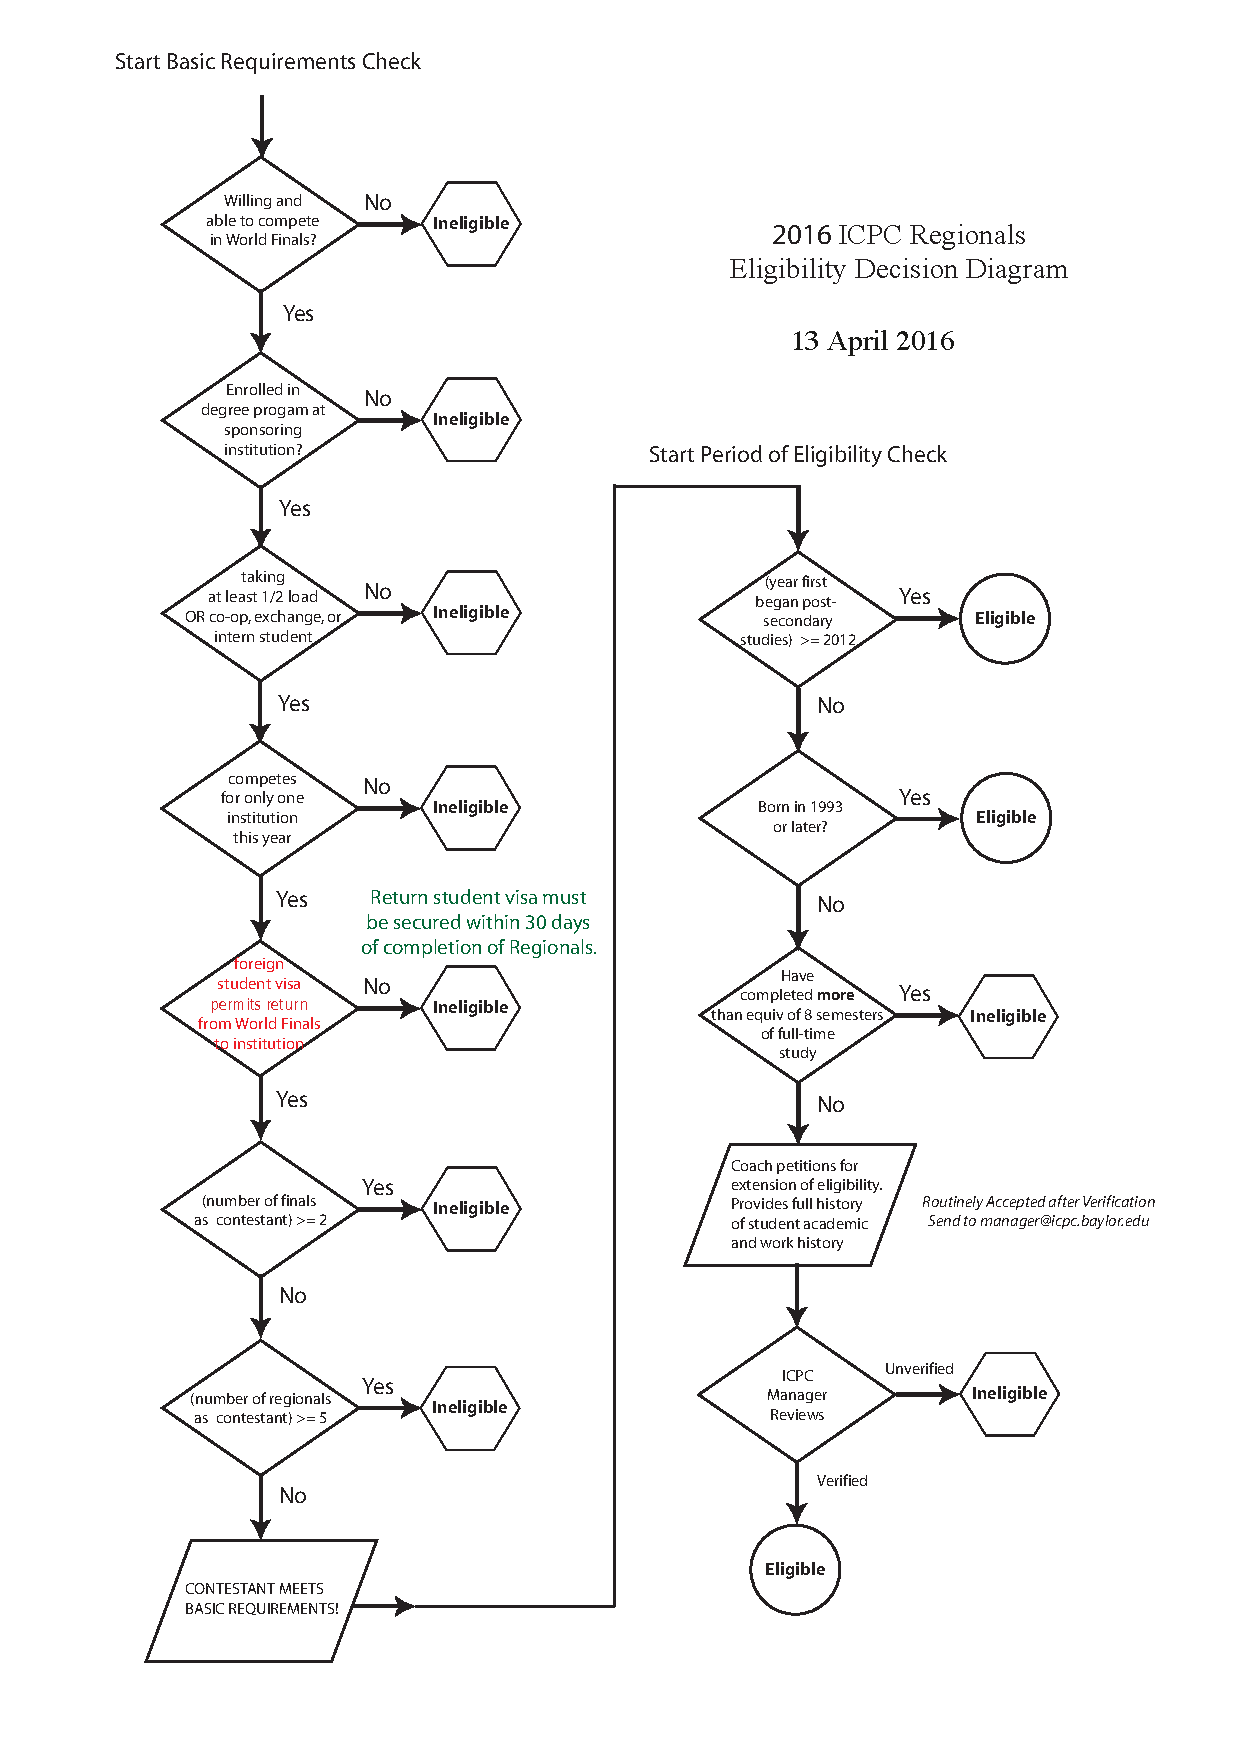
\includepdf[pages=-1]{./Attachments/EligibilityDecisionTree-2016.pdf}

\begin{center}
\vspace*{\fill}
This page is intentionally left blank.
\vspace*{\fill}
\end{center}
\clearpage

\section{DOMjudge team manual}\label{DJteam}
%\addcontentsline{toc}{section}{DOMjudge team manual}
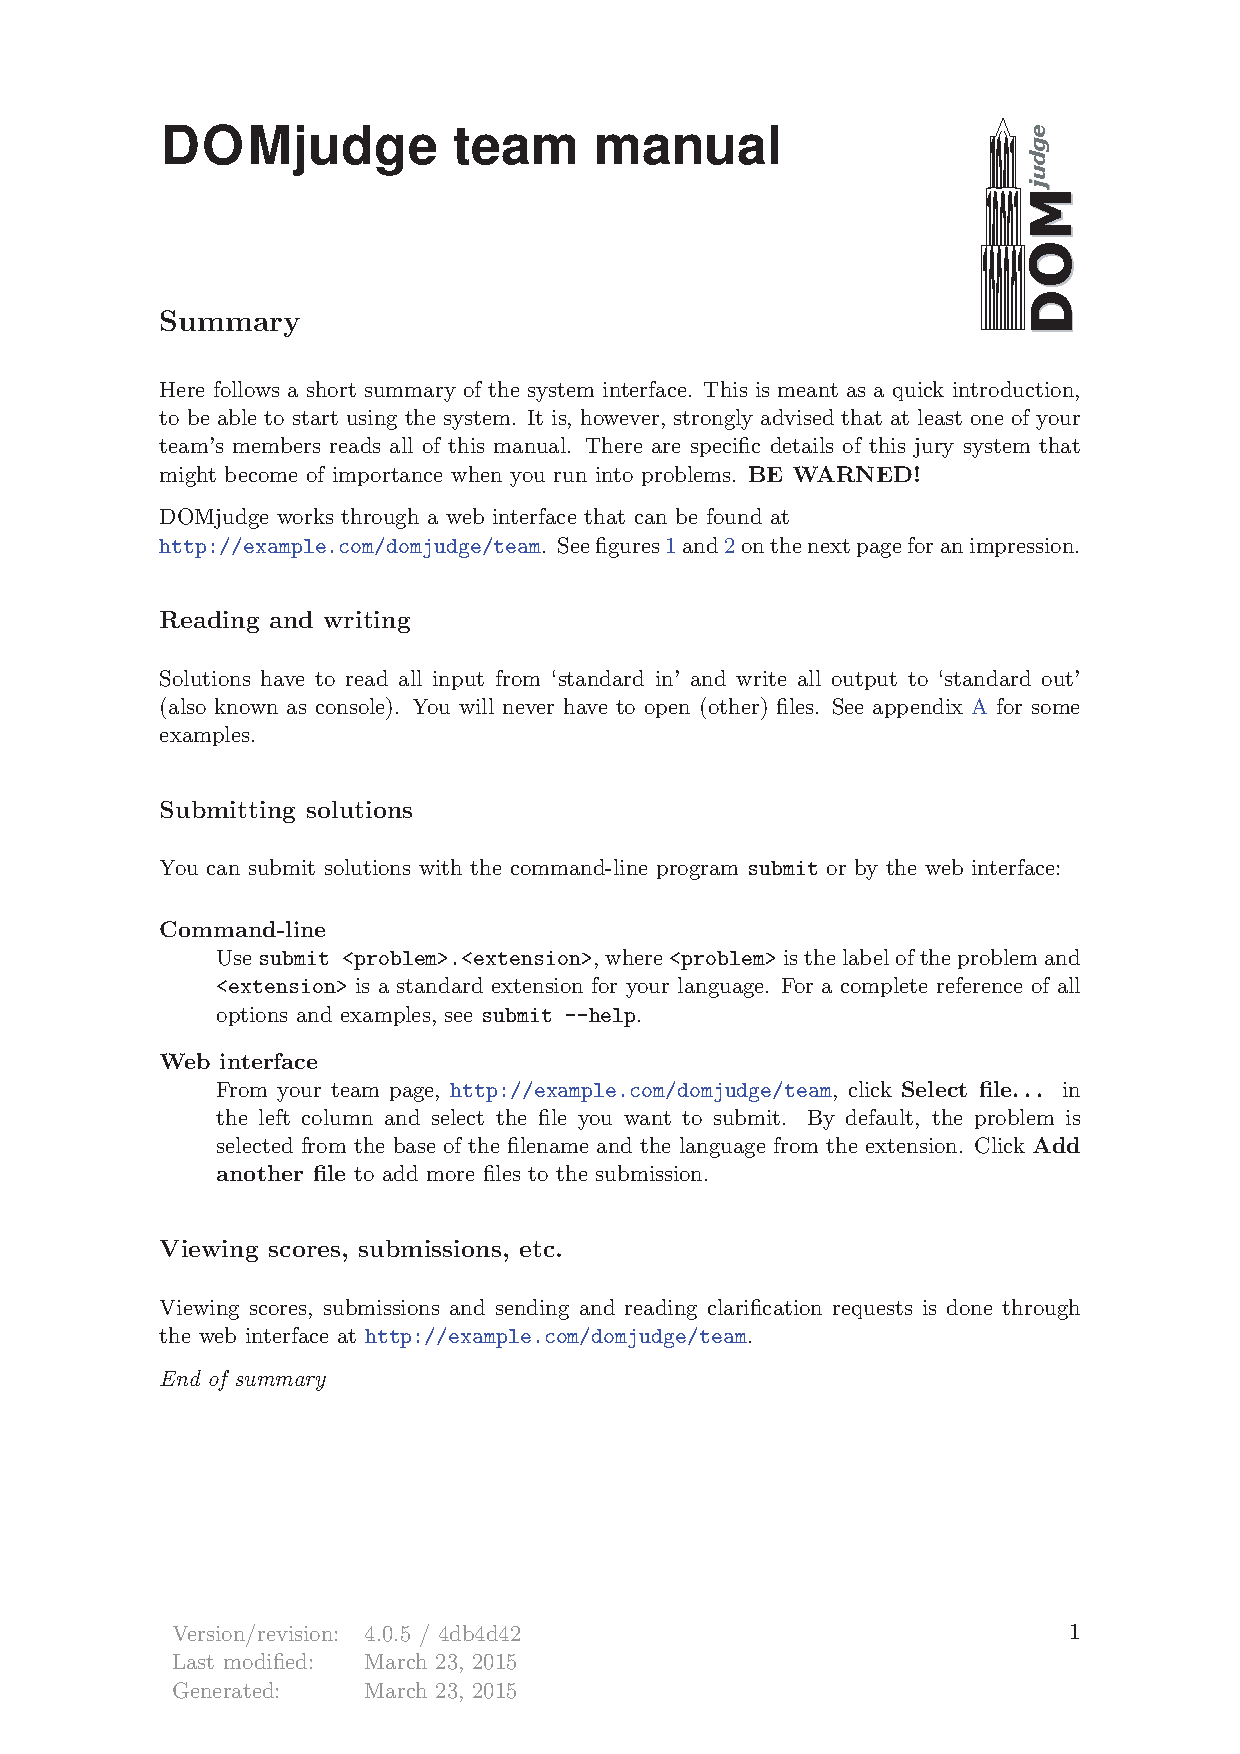
\includepdf[pages=-]{./Attachments/DOMjudge/team-manual.pdf}

\section{Amsterdam Algorithm Programming Preliminaries}\label{Rulebook}

\includepdf[pages=-]{./Attachments/Rules/AAPP_Rules_2016.pdf}
%
\includepdf[pages=1-3]{./Attachments/Rules/BAPC_Rules_2015.pdf} %pages=- (om alles in te laden van de PDF) geeft errors

\end{document}